\documentclass[11pt,a4paper]{report}
\usepackage{graphics,graphicx}
\usepackage{hyperref}
\usepackage{fullpage}
\usepackage{pdflscape}
\usepackage{tikz}
\usepackage{setspace}
\usepackage{enumitem}
\usepackage{index}
\usepackage{gantt}
\makeindex
\onehalfspacing

\usepackage{graphicx}
\begin{document}

\title{Interactive Graduate Student Information Database: Midterm Report} 
\author{Kartik Thakore (250313003)\\kthakore@uwo.ca}
\maketitle

\tableofcontents
\clearpage
\newpage
\chapter{Software Specifications}
\section{Introduction}
\index{purpose}
\subsection{Purpose}
The purpose of this report is to document preliminary elicited requirements for the Interactive Graduate Student Information System (SIMS). Additionally, in accordance with the Agile project management
methodology, a walk through of the first iteration is documented. Our first iteration includes two system
critical features which will be used for iterative system development of the system. Database schemas and
operational logic for user authentication and calculations for graduate student funding were accomplished.
A database schematic was designed after performing extensive analysis based on our specifications, data flow
requirements and approved system critical assumptions. Data normalization was performed and a Representational State Transfer (REST) framework was implemented to combine components. Furthermore, unit and
integration testing were performed with the preliminary implementation in place. For preparation of future
iterations, a sign-off from end users and client is required. However, we have started the rapid prototyping
of the e-signature component for the advisory meeting tracking feature.
\subsection{Scope}
\index{scope}
\index{BioMedical Physics}
The scope of the following requirements is to provide a pilot software back end for the BioMedical Physics
Graduate program at UWO. First the system will replace the current method of tracking student information
pictured in Figure \ref{fig:Curr_Sys}.
\begin{itemize}
\item The current system provides the following features which directly fall into scope for this product:
\begin{itemize}
\item Storage of Intrinsic Student Value
\item Graphical User Interface for Entering Student Data
\item Saving portable reports for external users
\end{itemize}
\item The new system will additionally need to address the following concerns:
\begin{itemize} 
\item Store data securely and with more redundancy
\item Simply the User Interface for using the system
\item Remove the load of managing data solely on one user
\item Allow faculty members to view data in a meaningful way
\item Allow students to update their information
\item Allow advisory committee members to store and retrieve signatures and comments on the system
\end{itemize} 
\end{itemize}
Currently the scope is limited to tackling these core issues. However since the project cycle is iterative,
the scope can be expanded in a controlled manner, should the situation demand it.
\subsection{Definitions, acronyms, and abbreviations}
\begin{itemize}
\item SIMS: Student Information System
\item UWO: University of Western Ontario
\item REST: Software Architecture for Web Applications
\item VPN: Virtual Private Network
\item SSL: Security Protocol for Web Applications
\item SRS: Software Specifications Document 
\item SDS: Software Design Document 
\end{itemize}

\subsection{Overview}
The SIMS core is a secure application that aims to be flexible to handle business rules of varying graduate
student programs. In the scope of this project however, focus will be placed on the Graduate Student
Program at the BioMedical Physics program at University of Western Ontario. At the very least SIMS
will hold graduate student, funding and advisory meeting data. Additionally SIMS will allow the program
administrator to organize collected data into reports and to send automatic request for data to students.
Also advisors and other faculty users will be able to see student data, progress and any advisory meetings
they have attended. SIMS will also place an emphasis on providing security of student personal data and
faculty identifications. Overall SIMS, will be replacing the current manual system of tracking students and
their progress through graduate programs.
Figure \ref{fig:New_Sys} shows the overview of the required system. The user will access the system via the Client and
Tablet devices. The data from the tablet will be processed in the client and sent via the TCP/IP protocol
to the Application Server (AppServer). The responsibility of the AppServer is to provide secure access, and
host the application. The AppServer will communicate with the Services Server to add triggers and use the
database. The AppServer and the ServicesServer will be located on a local network which is accessed via
a Virtual Private Network (VPN). Figure 3 models the users of the SIMS system. The user groups can be
broken down into 3 categories, the Student, the Faculty and the Technical Administrator. The technical
administrator will have access only to the authentication data. While the student and the faculty will have
access only to the tracked data. Additionally the faculty will have more access over the student. The role
and operations requirements will be covered more in-depth in the system features.
\begin{figure}[htp]
\centering
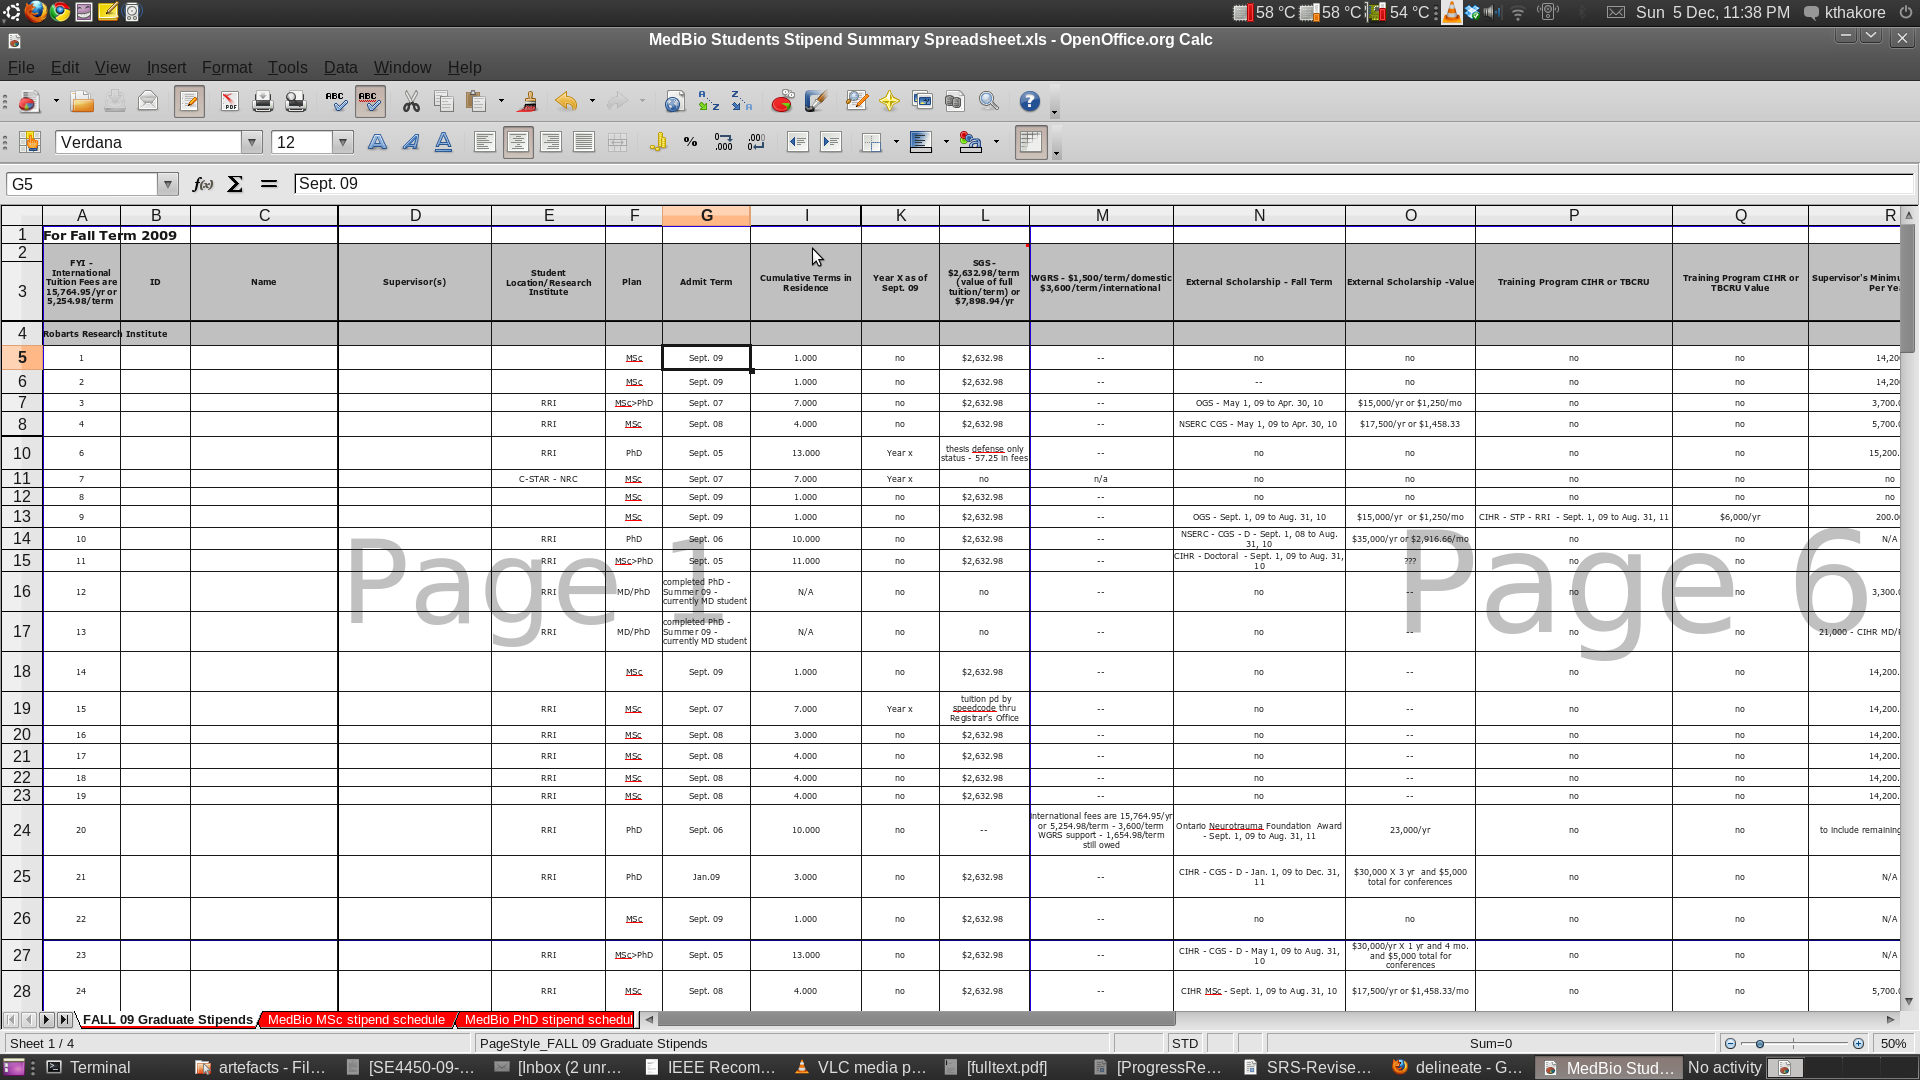
\includegraphics[scale=0.25]{diagrams/Current_System.png}
\caption{Current System}
\label{fig:Curr_Sys}
\end{figure}

\begin{figure}[htp]
\centering
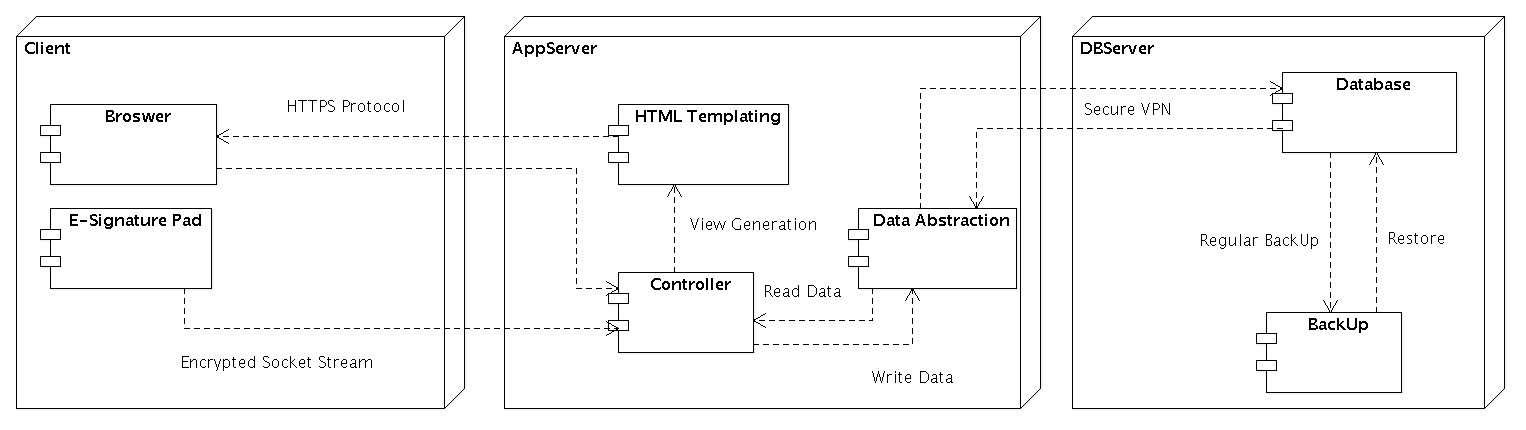
\includegraphics[scale=0.40]{diagrams/SystemOverview.png}
\caption{Proposed System}
\label{fig:New_Sys}
\end{figure}



\section{Overall Description}

\subsection{Product perspective}
The product will be self contained as it is responsible form User Interface, Application and Data Storage.
Figure \ref{fig:New_Sys} again describes the perspective of the system.
The product will have the following constraints:
\begin{itemize}
\item User Interface: The specifications of each view of the user interface will be provided for this project.
\item Hardware Interface: The system will be using a Wacom tablet as a hardware to acquire signatures.
\item Software interfaces: The system will have to employ several software interfaces.
\begin{itemize}
\item Application Server: Apache 2.0 will be used to deploy the system with SSL security.
\item VPN Provider: OpenVPN will be used to deploy our system as a self contained virtual private
network.
\item Database Software: A PostgreSQL RDBMS server will be used to run our Data Storage Component of the Software.
\end{itemize}
\end{itemize}
\subsection{Product function}
\subsection{User characteristics}
Figure \ref{fig:users} describes the relation between the users of the systems, for further clarification:
\begin{itemize}
\item General User: Any user of the system, can login into the system 
\begin{itemize}
\item Faculty: Members of the faculty that can see data of several students who are not student themselves
\begin{itemize}
\item Graduate Administrator: Essentially the super user of the system, can access and modify all data 
\item Advisory Committee Member: Can view attached student data and advisory meeting documents
\item Graduate Faculty Executives: Can view all student data and view publish reports 	
\end{itemize}
\item Technical Administrator: A user that cannot access any data but can manage users 
\item Graduate Student: A student that can only view their own information and update it
\end{itemize}
\end{itemize}

\begin{figure}[htp]
\centering
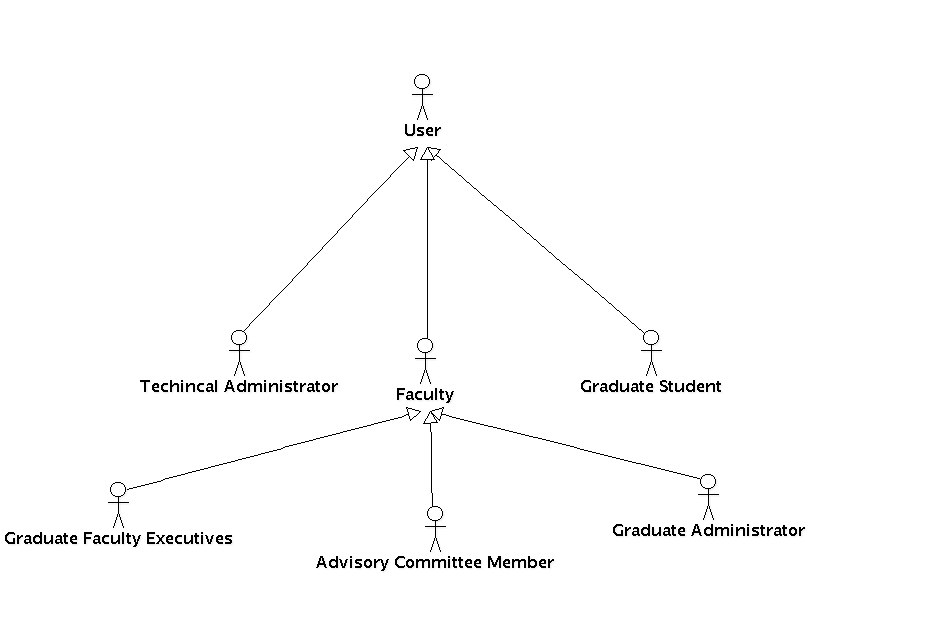
\includegraphics[scale=0.40]{diagrams/use_cases/UserHeirachy_uc.png}
\caption{Users of the System}
\label{fig:users}
\end{figure}

\subsection{Constraints}

\subsubsection{Technical Environment}
SIMS will be built on the Linux Server platform for the Database and Application Server. The client will be limited to a Linux Operating System with the Firefox 3.6 web browser.  
\subsubsection{Security}
UWO has strict guidelines (FIPPA) to handling signatures and student data. For this purpose proven technologies will be used, such as HTTP secure and VPN.
\subsubsection{Reliability of Data}
Data in SIMS is critical and needs to be protected from data losses. A regular backup of the database will help to accomplish this. 

\subsection{Assumptions and dependencies}
\subsubsection{Student Data v.s User Data}
Student Data is separate from the system, and will not be removed from the system after they graduate. However a user can still be expired from the system. Since archival is needed for a period of atleast 7 years SIMS will need to seperate user access and student data. 
\subsubsection{Intrinsic Student Data}
Another assumption required by SIMS's requirement is that Student can only be stored in the system if they have a funded term attached to them. This implies that funding is tied on a term basis, which can help to simply futher calculations. 

\section{Specific Requirements}
\subsection{External interface requirements}
\subsubsection{Graphical User Interface}
A set of graphical user interfaces defined in HTML will be provided for the system to template. SIMS will show the interfaces as is and add dynamic data to them. 
\subsubsection{Hardware Interface}
SIMS will acquire signatures from client side wacom tablets from a USB 2.0 protocol. Data will be output as a BMP file format. 

\begin{figure}[htp]
\centering
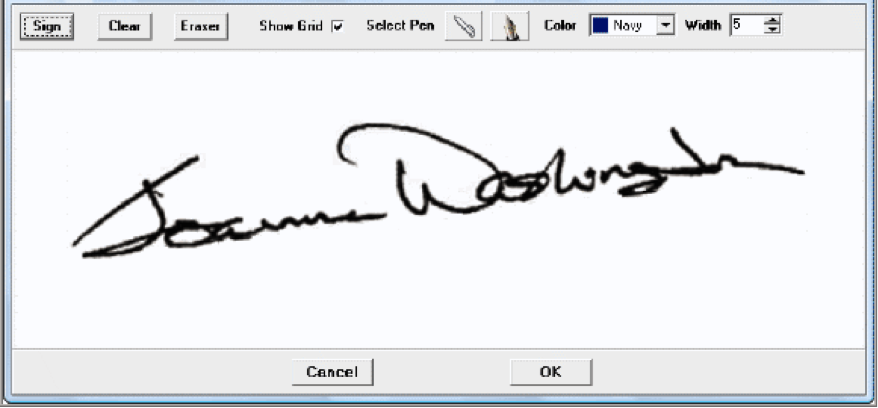
\includegraphics[scale=0.75]{diagrams/HTMLTemplating/Figure6.png}
\caption{Signature Interface View}
\label{fig:signature}
\end{figure}

\begin{itemize}
\item Purpose: To provide an interface for recording advisory committee member signatures.
\item Response Sequence: When the e-signature pad is connected to the device, it will automatically start the e-signature interface which records an individual signature.
\item Associated Functional Requirements:
\begin{itemize}
\item Clear: Ability to clear the signature if the signer does not accept the signature
\item Sign: Once the output on the screen is satisfactory, the user can "Sign" the document which will save the image in a document on the database.
\end{itemize}
\end{itemize}
\subsection{Functional requirements}
\subsubsection{User Administration}

\begin{figure}[htp]
\centering
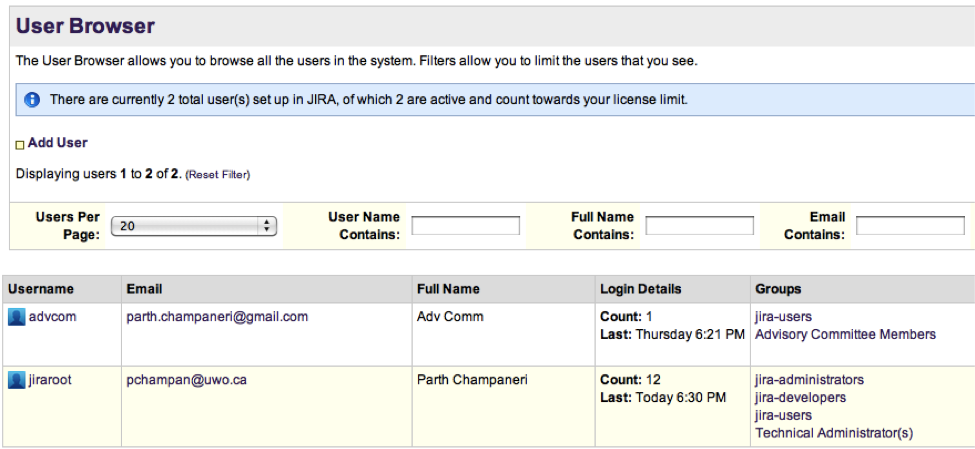
\includegraphics[scale=1]{diagrams/HTMLTemplating/Figure7.png}
\caption{User Browser}
\label{fig:UserBrowser}
\end{figure}


\begin{itemize}
\item Purpose: The user browser lists all the users in the system for technical administration. 
\item Response Sequence: Login and click on User Browser from the admin. From this page, the administrator can perform the following functions:
\item Associated Functional Requirements:
\begin{itemize}
\item Create new users: Adding a new user to the system can only be accomplished by the technical administrator after an approval from the Graduate Administrator.
\begin{figure}[htp]
\centering
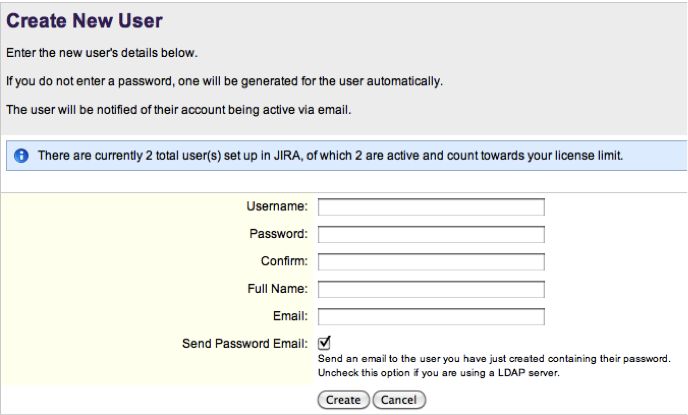
\includegraphics[scale=1]{diagrams/HTMLTemplating/Figure8.png}
\caption{New Users}
\label{fig:NewUser}
\end{figure}
\item Adding new user roles: User roles are primary stakeholder groups for the system. Currently, our primary stakeholders are Advisory Committee Members, Graduate Administrators, Graduate Executives, and Graduate Students.
\begin{figure}[htp]
\centering
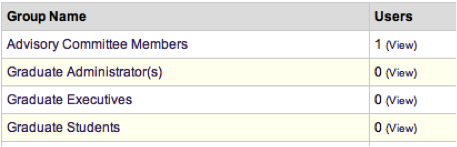
\includegraphics[scale=1]{diagrams/HTMLTemplating/Figure9.png}
\caption{New Users Roles}
\label{fig:NewUserRoles}
\end{figure}

\item Adding Operation to roles: Permissions can be added to the user permission list by clicking on the Add New permission button under User Administration. This can be done by the technical administrator.

\begin{figure}[htp]
\centering
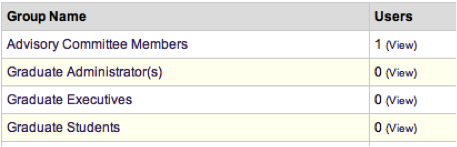
\includegraphics[scale=1]{diagrams/HTMLTemplating/Figure9.png}
\caption{New Operations}
\label{fig:NewPermission}
\end{figure}


\end{itemize}
\end{itemize}

\subsubsection{System wide login page}

\begin{figure}[htp]
\centering
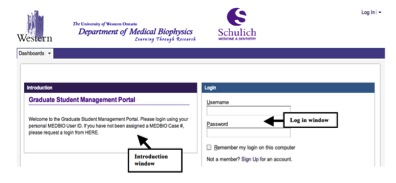
\includegraphics[scale=1]{diagrams/HTMLTemplating/Figure1.jpg}
\caption{System Wide Login Page}
\label{fig:SystemWideLogin}
\end{figure}


\begin{itemize}
\item Purpose: Provide a universal log-in page to provide access to the end users of the system
\item Response Sequence: In order to access the login page, user will have to type the system URL in a supported browser and will be directed to this log in page. 
\item Associated Functional Requirements: 
\begin {itemize} 
\item Introduction widget: This widget will provide a short introduction to the purpose of the management system. It will also feature an Important Links section with a link to the website of Department of Medical BioPhysics. Furthermore, a link to a technical troubleshooting page will be created.
\item Login window: This is the actual login page where the user will enter their credentials to login. Users cannot sign up for the system individually. The Graduate Administrator facilitates the sign up process and a direct link to request the login credentials will be set up.
\end{itemize}
\end{itemize}


\subsubsection{System Dashboard}
\begin{figure}[htp]
\centering
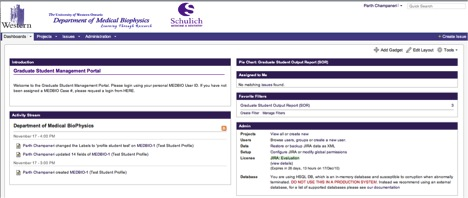
\includegraphics[scale=1]{diagrams/HTMLTemplating/Figure2.jpg}
\caption{System Dashboard Page}
\label{fig:SystemDashBoard}
\end{figure}

\begin{itemize}
\item Purpose: Provide a centralized location of all system functions while preserving ease of use and accessibility.
\item Response sequence: The user will be directed to this page after login.
\item Associated Functional Requirements:
\begin{itemize}
\item Provide various plugins on the dashboard based on different user roles and access for access to student profiles and various system features. Plugins can be RSS feed or activity stream, various preset charts and reports.
\item Search: Be able to search a students profile from the dashboard.
\end{itemize}
\end{itemize}

\subsubsection{Student Profile}
\begin{figure}[htp]
\centering
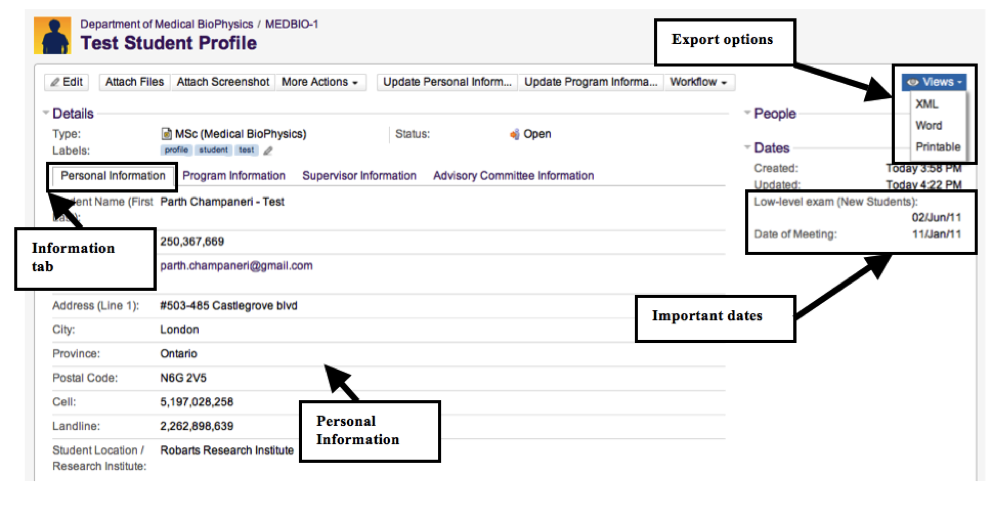
\includegraphics[scale=1]{diagrams/HTMLTemplating/Figure3.png}
\caption{Student Profile Page}
\label{fig:StudentProfile}
\end{figure}

\begin{figure}[htp]
\centering
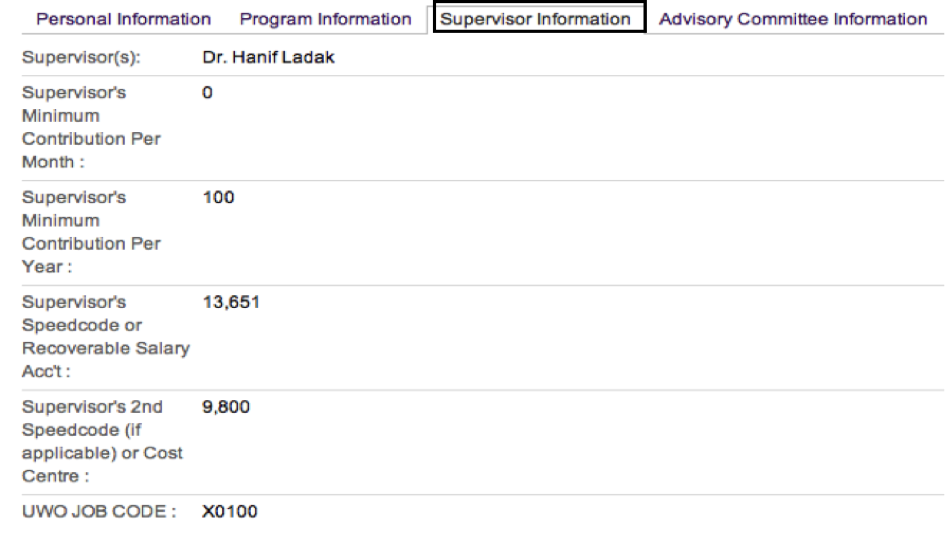
\includegraphics[scale=1]{diagrams/HTMLTemplating/Figure4.png}
\caption{Supervisor Information Page}
\label{fig:SuperInfo}
\end{figure}


\begin{itemize}
\item Purpose: Provide an intuitive dossier format interface for users to see the student profile in a centralized location. The key goal is to ensure that all the important system functionality in a centralized location. Note the attached sample HTML page.
\item Response sequence: In order to access the GUI, the user will be required to login and will be taken to a dashboard which will have options to generate reports and search a student by their assigned id. Once selected the user will be able to see a student profile and be able to perform various functions based on their authentication scope as defined in the access control list.
\item Associated Functional Requirements:
\begin{itemize}
\item Information Tab Section: The profile page will feature information tabs with centralized information about their Personal Information, Program Information, Supervisor Information and Advisory Committee Meeting Information.
\item Supervisor Information: This tab contains information regarding a students’ direct Supervisor Name and information about the supervisors minimum student contribution along with other logistical information. This information is created with the sample medical biophysics excel sheet provided by the Graduate Administrator user at the department of Medical BioPhysics.	

\item Expansion: Each section can be clicked on to show summary of additional information
\item Link:  Each information tab will link to another section pages (if applicable)
\item Grouping: Group dates and People in the same window area for better accessibility
Export Options: There should be an export option to ensure that a user can export their entire student profile in Word, PDF or in a Printable format
\item Attachment Options: The dossier should feature an attachment tab that includes all relevant attachments/forms for that student profile.
\end{itemize}
\end{itemize}

\subsubsection{Graduate Students’ Personal Information}
\begin{itemize}
\item Graduate Students’ Personal Information:
Contains data regarding to the students contact information including their UWO e-mail address and their current location. This system feature is to document how personal information is stored and accessed via different user roles. 
\item Graduate Students: Graduate Students can view their entire profile including their program information, supervisor information, advisory committee information and personal information. Data access is restricted only to their personal profile.
\item Graduate Administrator: Ability to edit all fields.
\item Graduate Executives and Advisory Committee members: Read Only access.
\item Update Personal information
\begin{itemize}
\item Visibility: Graduate students only
\item Restrictions: Only allowed to update contact information and address. 
\item Usability :Graduate administrator is responsible for inputting student data.
\end{itemize}
\end{itemize}
\subsubsection{Graduate Students’ Program Information}

\begin{figure}[htp]
\centering
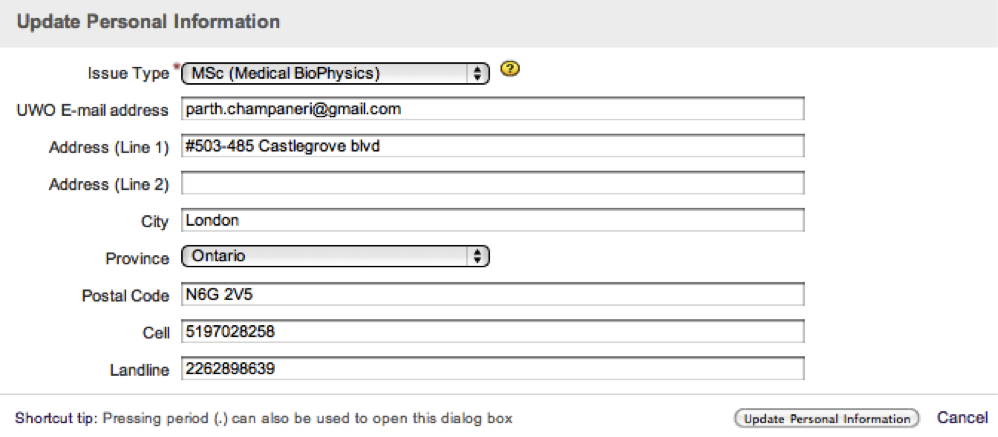
\includegraphics[scale=1]{diagrams/HTMLTemplating/UpdatePersonalInfoStudent.png}
\caption{Update Personal Information Student}
\label{fig:UpdatePIS}
\end{figure}

\begin{itemize}

\item Contains information related directly to the students program enrollment. Information includes Admission Term and Year, Thesis information, Publications (if any) and a custom field that records if the student has indicated MSc to PhD reclassification.
\item Update Program Information
\begin{itemize}
\item Visibility: Graduate students only
\item Restrictions: Allowed to update Publications, Thesis (if applicable) and Low-Level exam date if known. 
\end {itemize} 
\end {itemize} 

\subsubsection{Graduate Students’ Advisory Committee}
\begin{itemize}
\item Advisory Committee Information tab is a centralized location for all advisory committee information which has taken place for a student. Under this tab, pertaining information such as the list of all advisory meetings, evaluation of a particular advisory meeting whether it was satisfactory or unsatisfactory and any supervisor/member recommendations after the meeting. Advisory committee is a progression requirement which happens for each student atleast once a year. Scheduling is usually done by the student or by the graduate administrator. One of the key requirements is to track and remind students of their advisory meeting output and ensure that a post-meeting report is generated to satisfy their progression requirements.

\begin{figure}[htp]
\centering
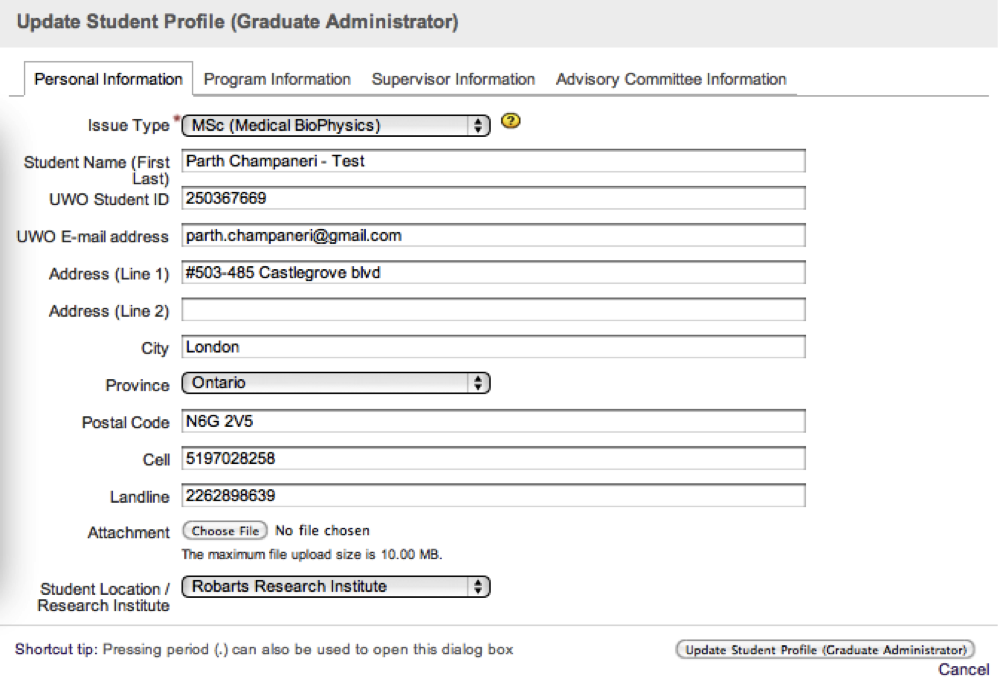
\includegraphics[scale=1]{diagrams/HTMLTemplating/UpdateStudentProfileAdmin.png}
\caption{Update Advisory Committee Information}
\label{fig:UpdateACI}
\end{figure}

\item Update Advisory Committee Information
\begin{itemize}
\item Visibility: Graduate students and Graduate Administrator
\item Restrictions: Allowed to update names of supervisor and advisors after a date for the meeting has been formed.
\end{itemize}
\item Comment on Advisory Committee Meeting:

\begin{figure}[htp]
\centering
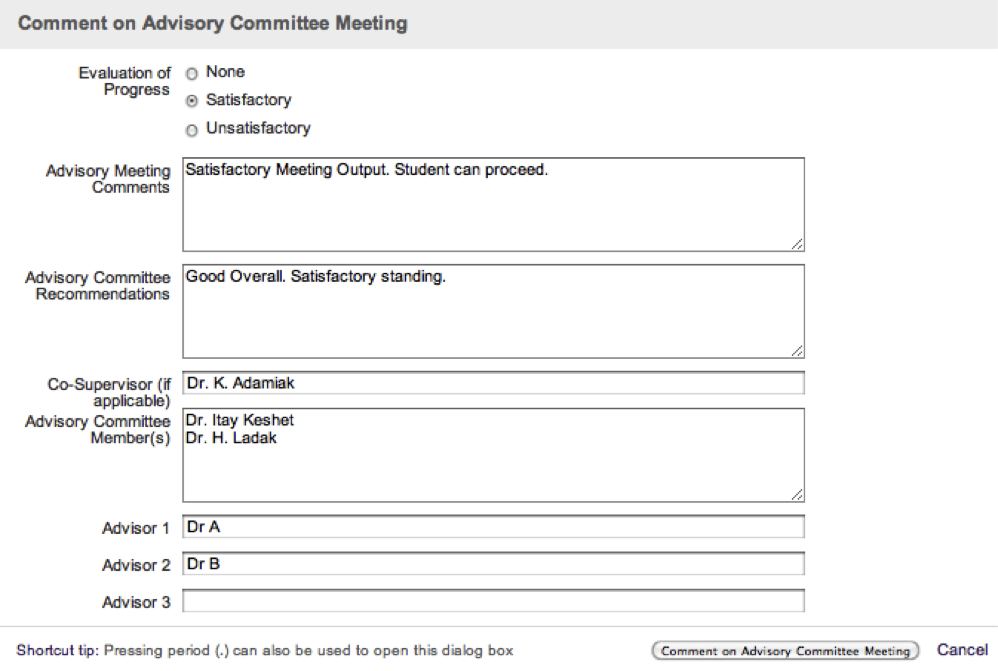
\includegraphics[scale=1]{diagrams/HTMLTemplating/CommentAdvisory.png}
\caption{Adding Comments to Advisory meetings}
\label{fig:UpdateCAM}
\end{figure}

\begin{itemize}
\item Visibility: Advisory Committee Members
\item Restrictions: Cannot access any other data. Members can update progress and output of the meeting. Can also provide recommendations and comments.
\end{itemize}
\end{itemize}

\subsubsection{Data Reporting}
\begin{itemize}
\item Queries: Reports can be generated by filtering via various fields or by entering customized queries in the reporting interface.
\item Queries can be run by the administrator, advisory members and graduate executives.
\item Sample Student Profile Report (Word): Users can export student profile in a Word document which contains all the information regarding the selected student. The scope of the document generated will be restricted to the roles and permission of the user.
\item Sample Graduate Student Output Report (SOR) - Excel: Users can export a SOR based on custom queries which are either preset or custom created.

\begin{figure}[htp]
\centering
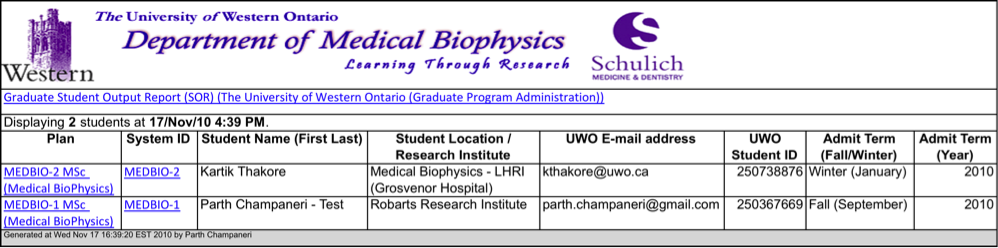
\includegraphics[scale=1]{diagrams/HTMLTemplating/SOR_Excel.png}
\caption{Excel Graduate SOR Report}
\label{fig:ExcelSOR}
\end{figure}

\item Custom Pie Charts: Pie charts and trend charts can be generated based on the SOR or a custom query.

\begin{figure}[htp]
\centering
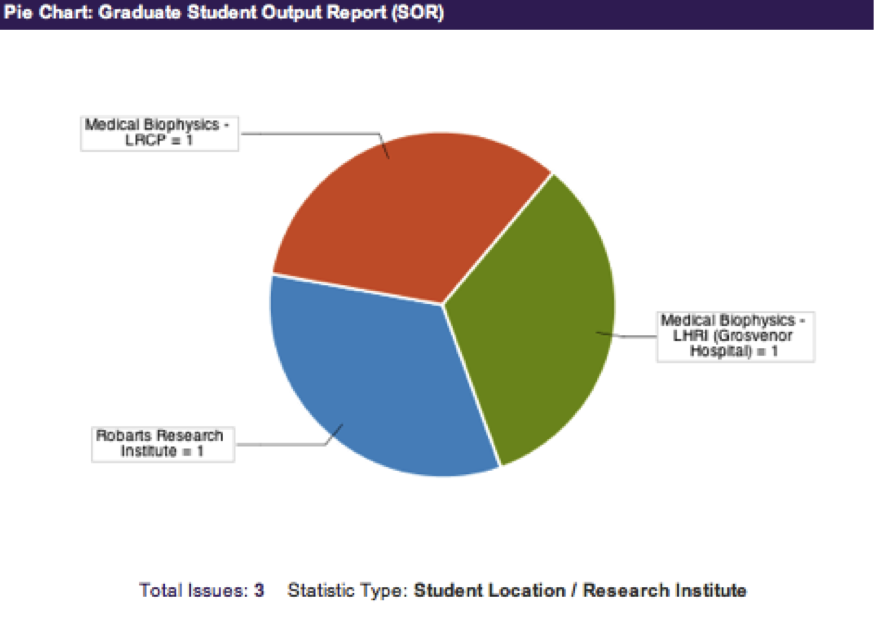
\includegraphics[scale=1]{diagrams/HTMLTemplating/PieChart.png}
\caption{Excel Graduate SOR Pie Chart}
\label{fig:PieSOR}
\end{figure}

\end{itemize}

\chapter{Design}
\section{Iteration 1}
During iteration 1 of the project, the tasked was focused on the 
\section{Analysis}

\subsection{User Hierarchy}
As specified in the SRS the user hierarchy is well defined in Figure \ref{fig:users}. Looking at the user interface provided the following use cases can be 
defined.

\subsection{Use Cases}

\subsubsection{Generic User}

\begin{figure}[htp]
\centering
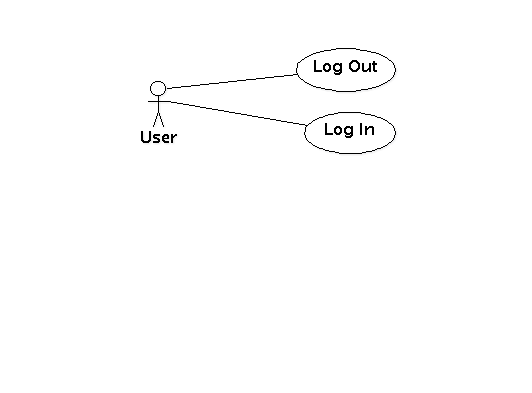
\includegraphics[scale=0.5]{diagrams/use_cases/User_uc.png}
\caption{User Login and Logout}
\label{fig:UserLog}
\end{figure}



\subsubsection{User Administration}

\begin{figure}[htp]
\centering
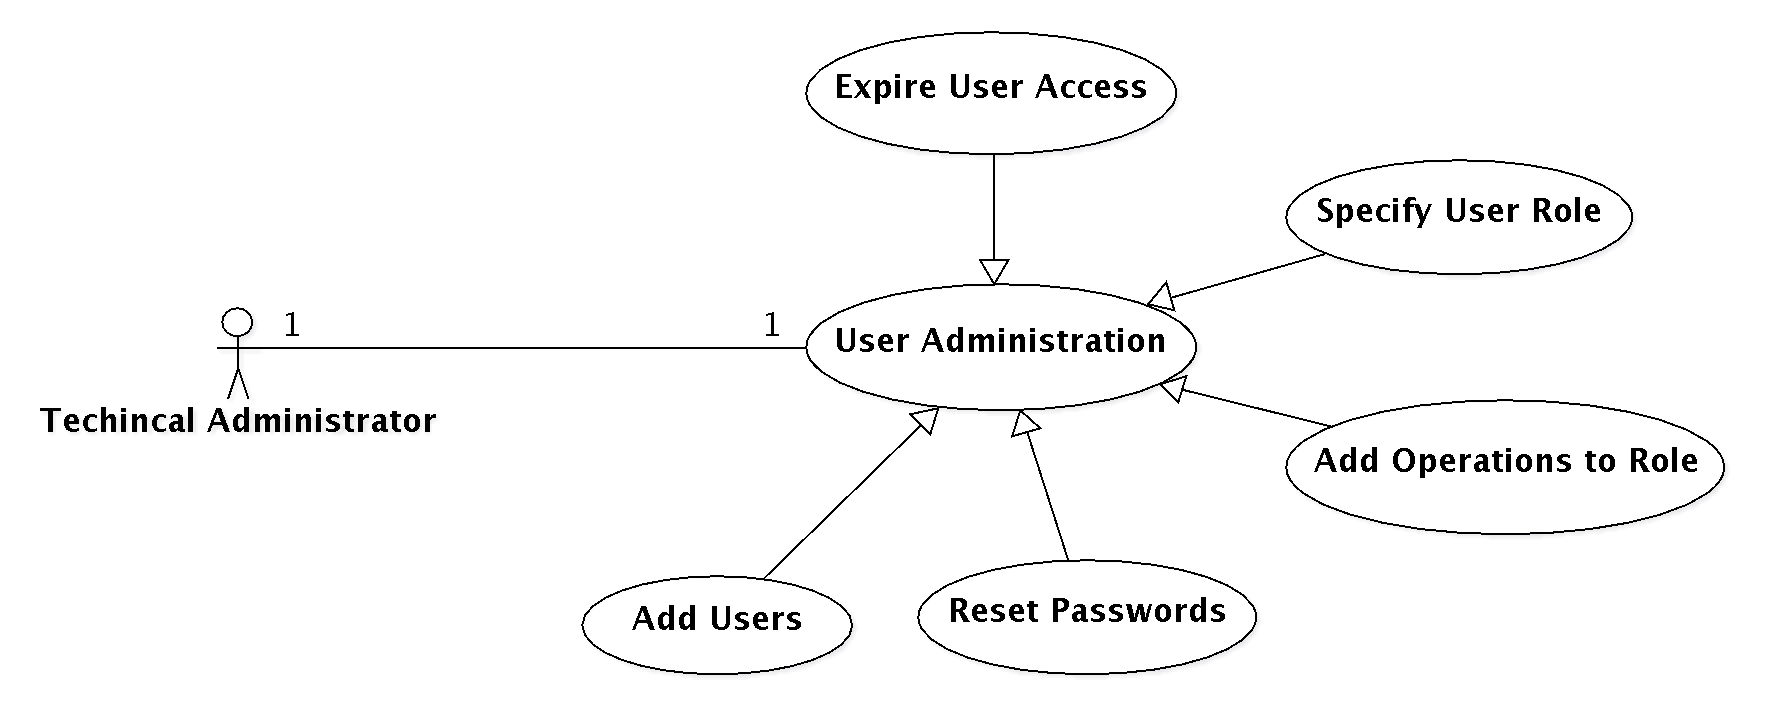
\includegraphics[scale=0.5]{diagrams/use_cases/TechAdmin_uc.png}
\caption{User Administration}
\label{fig:UserAdmin}
\end{figure}

\subsubsection{Student Access}
\begin{figure}[htp]
\centering
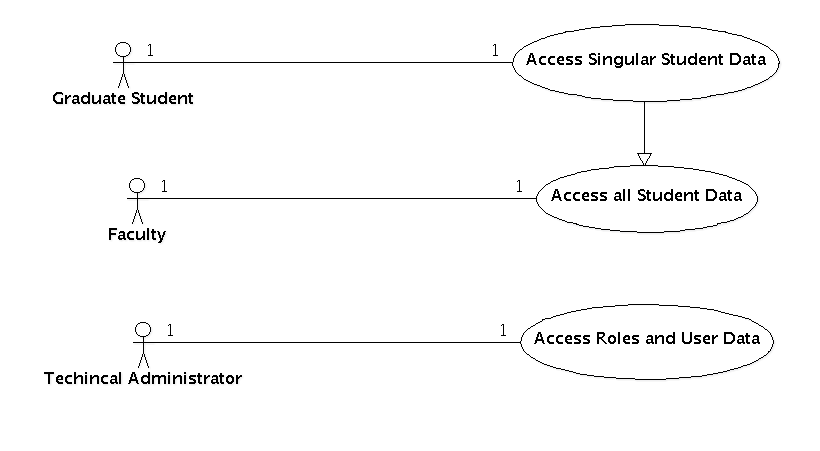
\includegraphics[scale=0.5]{diagrams/use_cases/access_uc.png}
\caption{User Access}
\label{fig:UserAccess}
\end{figure}


Iteration one focused on two major use cases Figure 

-> Content Analysis 
Content Relationships and Hierarchy 

-> Interaction diagrams
	Student State Chart 
	Use Cases to State Chart 

\section{Design}
\subsection{Goals}

-> Simplicity

-> Consistency

-> Robustness

-> Ease of Use

\subsection{Component Design}
Student ER diagrams
Role Based Authentication
Perl Framework 
Client Design 
\subsection{Architecture Design}
Using MVC Architecture 
\section{Implementation}

\subsection{Catalyst Framework}

\section{Testing and Feedback}

\section{Future Work}
\subsection{HTML Templates}
\subsection{Server Configuration}
\subsection{Advisory Committee Meeting}
\chapter{Walk through}
\section{Concerns}
\subsection{Organization}

\section{Report \& Follow up}
\subsection{Structure in Design}

\chapter{Partial Test Plan}
\section{Unit Testing}
\section{Integration Testing}
\section{Performance Testing} 
\chapter{Updated Gantt Chart}
\begin{landscape}
	\scalebox{0.8}{
		\begin{gantt}[xunitlength=0.65cm,fontsize=\small,titlefontsize=\small,drawledgerline=true]{16}{32}
		\begin{ganttitle}
		\titleelement{2010}{16}
		\titleelement{2011}{16}
		\end{ganttitle}
		\begin{ganttitle}
		\titleelement{Sept}{4}
		\titleelement{Oct}{4}
		\titleelement{Nov}{4}
		\titleelement{Dec}{4}
		\titleelement{Jan}{4}
		\titleelement{Feb}{4}
		\titleelement{Mar}{4}
		\titleelement{Apr}{4}
		\end{ganttitle}
		\begin{ganttitle}
		\numtitle{1}{1}{4}{1}
		\numtitle{1}{1}{4}{1}
		\numtitle{1}{1}{4}{1}
		\numtitle{1}{1}{4}{1}
		\numtitle{1}{1}{4}{1}
		\numtitle{1}{1}{4}{1}
		\numtitle{1}{1}{4}{1}
		\numtitle{1}{1}{4}{1}
		\end{ganttitle}
		\ganttbar{Problem Definition}{1}{3}
		\ganttbar{Requirements Engineering}{4}{2}
		\ganttcon{4}{3}{4}{4}
		\ganttbar{Authentication and Student Funding Feature}{6}{3}
		\ganttcon{6}{4}{6}{5}
		\ganttbar{Authentication and Student Funding Feature: Feedback}{10}{1}
		\ganttcon{9}{5}{10}{6}
		\ganttcon{9}{5}{9}{7}
		\ganttbar{Advisory Meetings Feature}{9}{3}
		\ganttbar{Adivsory Meetings Feature: Feedback}{12}{1}
		\ganttcon{12}{7}{12}{8}
		\ganttcon{12}{7}{12}{9}
		\ganttbar{Iteration 3}{12}{3}
		\ganttbar{Iteration 3: Feedback}{16}{1}
		\ganttcon{15}{9}{16}{10}
		\ganttcon{15}{9}{16}{11}
		\ganttbar{Iteration 4}{16}{3}
		\ganttbar{Iteration 4: Feedback}{19}{1}
		\ganttcon{19}{11}{19}{12}
		\ganttcon{19}{11}{19}{13}
		\ganttbar{Iteration 5}{19}{3}
		\ganttcon{22}{13}{22}{14}
		\ganttbar{Acceptance Testing}{22}{2}
		\ganttcon{24}{14}{24}{15}
		\ganttbar{Project Documentation}{24}{4}  
		\end{gantt}
	}
\end{landscape}
\chapter{References}

\begin{verbatim}
Joe Lin, Charley Ho, Wasim Sadiq, and Maria E. Orlowska, "On workflow enabled e-learning 
services", Advanced Learning Technologies, IEEE International Conference on,
vol. 0, pp. 0349, 2001.

Office of the Privacy Commissioner of Canada, "Canada's personal information protection 
and electronic documents act", http://www.priv.gc.ca/information/guide_e.cfm, 2003, 
This is an electronic doc- ument. Date of publication: November 20, 2003. 
Date retrieved: October 4, 2010.

T.G. Zimmerman, G.F. Russell, A. Heilper, B.A. Smith, J. Hu, D. Markman, J.E. Graham, 
C. Drews "Retail Applications of Signature Verification",
SPIE Defense and Security Symposium, Biometric Technology for Human Identification
, Orlando, Florida, April 2004.

Lidstrom, Mattias. "The Input Race: A comparative study between two input modalities." 
Luleå University of Technology. 28 May 2007. Department of Music and media. 10 Nov. 2010 
<http://epubl.ltu.se/1402-1552/2007/110/LTU-DUPP-07110-SE.pdf>

Bennett, William E. (Mahopac, NY), Boies, Stephen J. (Mahopac, NY), Davies,
 Anthony R. (Romsey, GB2), Etzold, Karl-friedrich (Briarcliff Manor, NY), Rodgers, 
 Todd K. (Chappaqua, NY) 1991 Optical stylus and passive digitizing tablet data 
 input system United States International Business Machines Corporation (Armonk, NY)	5051736 http://www.freepatentsonline.com/5051736.html

"Council highlights",	http://www.cou.on.ca/News/News---Views/Newsletters/PDFs/ 
Council-Highlights-2005May.aspx, 2005, 
This is an electronic document. Date of publication:
 May 1, 2005. Date retrieved: Sept 29th, 2010.

I.P.W. Fung, "On monitoring study progress with 
time-based course planning", Advanced Learning Technologies, 2001. Proceedings. 
IEEE International Conference on, pp. 361 –364, 2001.
\end{verbatim}


\clearpage
\newpage 

\listoffigures

\clearpage
\newpage 

\printindex

\end{document}
